\chapter{Introduction}
\label{Ch1}
%\setcounter{page}{1}
\pagenumbering{arabic}

\bigskip
\bigskip
\bigskip

This chapter presents the introduction of the thesis that includes the brief description of BlockChain, and the adopted approach to address the problems. This chapter also presents the scope of this thesis and the contributions of the thesis.

Image integrity is the task of checking if the image file's bits are changed or not at any point. A digital file might change by platforms. This would be fully online system. Nowadays with increasing people in digital world the editing softwares are getting smart. Most of the files that might be non-editable in some operating systems or file systems, but the so called hackers or masters of electronic devices have file systems that can easily access and change any file data. So in that way the media files can not be checked for integrity. And also while the images are shared in different platforms, the files' data might be changed according to their protocols for data compression or security.

The proposed system in this thesis will help us to detect those shared files and compare them not bit by bit, but context wise and signature wise. That means if one shares an image both our system as well as one of those online platforms and download them as separate file and check in our system, it should return truth values if data portion are same or atleast 95\% same. The system we are introducing the social media like platform that have the capability to store images and show them in news feed. There is a option for every photo to download in user's computer or mobile devices and after sharing and getting back the person can check if the file is intact or not in our proposed system by the digital signature.

\section{Scope of Discussion}
This thesis focuses on building a hybrid architechture inspired by one of the major implementations of BlockChain i.e. BitCoin~\cite{nakamoto2008bitcoin}. By the advancement of PHP (Hypertext PreProcessor) and JS (JavaScript) which are the basic building languages or platforms that can be run in any modern devices, it might be quite easy to make a peer-to-peer web-api (Application Programming Interface) running like bitcoin decentraized network as well as social media platform that might be a real Truth Machine. While comparing image files data we will first compress the data using our own protocol and compare by bit matching Euclid, or Deep CNN (Convolutional Neural Network).

\section{Methodological Approach}
The system that we are trying to build is capable of processing, storing and showing image files. Not only that, it also allows viewers to veryfy his own copy of the image. It is not easy to store and veryfy in a moment and it is about impossible to change the whole blockchain, because the miners have their own copy of the public ledger and their processed computation powers in their computers. The automated server should back up its data from both the Virtual miners as well as remote miners' computers. The studied and inspired technologies are discuussed in the thesis.

\section{Thesis Contribution}
The main contributions of this thesis includes
\begin{enumerate}
\item Proposes an user anonymity-preserving algorithm to be a part of Video Integrity Program.
\item Formally analyzes the security of the newly designed protocol as well as its performance.
\item The scheme, as compared to the existing schemes, not only authenticates the users but, also establishes a session key between the user and the System after successful mutual authentication.
\item The scheme provides many security and robustness features of user authentication and Block Processing scheme for BCTs.
\item No installation required to be a part of the system, except you want to be the miner.
\end{enumerate}

\section{Roadmap of the Thesis}
The structure of the thesis is as follows:
\begin{enumerate}
\item The Chapter \ref{Ch1} is an introductory part which discusses the scope of the thesis, about the contribution of this thesis and the motivation for writing it.
\item The Chapter \ref{Ch2} provides the background of Image integrity security aspects of it and previous works.
\item The Chapter \ref{Ch3} introduces the proposed authentication framework after highlighting the motivations behind this work.
\item The implementation of Chapter \ref{Ch5}, where an informal implementation of the proposed protocol has been discussed.
\item The Chapter \ref{Ch6} comprises of the conclusion and further work of the Project in future.
\end{enumerate}

\section{BlockChain}
A BlockChain or \textbf{\q{The Truth Machine}} ~\cite{the_truth_machine} can be broadly described as a peer-to-peer network of nodes that makes a collaborative effort in sensing certain specified chain of blocks of data around its periphery and thereby controls the surrounding environment.
Accrrding to Wikipedia~\cite{blockchain_wiki} a blockchain, originally block-chain, is a growing list of records, called blocks, which are linked using cryptography. Each block contains a cryptographic hash of the previous block, a timestamp, and transaction data (generally represented as a Merkle tree).
In BlockChains, each node consists of processing capability, it may contain multiple types of memory like program, data and memories, having a Web-Service transceiver, Client-side processors, and a power source. The nodes communicate with each other using web-services and self-organized.
There are certain nodes called miners that veryfies each transactions or entry of data in the chain and are the most reliable personnel in the network who always have the updated copy of blocks of data.

\begin{figure}
\begin{center}
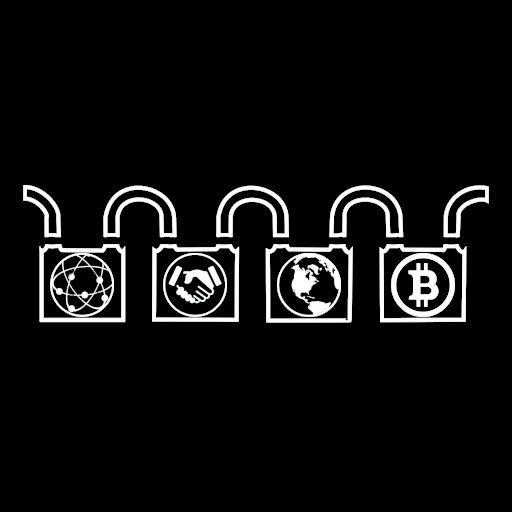
\includegraphics[width=0.5\textwidth]{./img_src/blockchain.jpg}
\end{center}
\caption{Overview of Block-Chain Technology (BCTs).}
\end{figure}

Some of the underlying concepts of the BlockChain especially BitCoin (the most popular implementation of BlockChain) and some other important technology are briefed.

\subsection{Peer-to-Peer Network}
This is the internet protocol that connects different logged in users as a node which is having some computation power. The users who are only uploading and verifying may have computer or smartphone, but the verifiers or the miners must have to work on computer with sufficient amount of computation power.

\subsection{Transactions}
Everything in crypto-currency comes under transactions, i.e. someone is sending some amount of money to someone else at some time. So a basic or overall transaction data can be structured as,

\fbox{\colorbox{lightgray}{\parbox[b][4cm][c]{0.50\linewidth}{
\textbf{\texttt{\noindent Transaction :: \{\\
\hspace*{1cm} \textless Transaction\_id\textgreater,\\
\hspace*{1cm} \textless TimeStamp\textgreater,\\
\hspace*{1cm} \textless Sender\_Id\textgreater,\\
\hspace*{1cm} \textless Receiver\_Id\textgreater,\\
\hspace*{1cm} \textless Amount\_Unit\textgreater\\
\noindent \}}}
}}}

This transaction details is send to every peer to verify. If they heard already about it, it is true, or it is false (same as women's un-manipulated gossip in village). If more than 50\% population declare it true, then it is allowed to be in the Public Ledger.

\subsection{Public Ledger}
This is the publicly shared record of transactions kept as a list of blocks. At a particular point of time everybody (every node), who are connected to the network, should have a same copy of ledger in their own devices of what server has. Whenever a new person logs into the network aotomatically the server forces to update the ledger to the person's device. So basically the ledger is the chain file.

\subsection{Chain of Blocks}
It means list of blocks of data having some common part with previous and next block. This is like Single-way linked-list(every node consists of data and program memory address to the next node). Every block contains a number of transactions and many more things.

\fbox{\colorbox{lightgray}{\parbox[b][6cm][c]{0.75\linewidth}{
\textbf{\texttt{\noindent Block :: \{\\
\hspace*{1cm} \textless Block\_Id\textgreater,\\
\hspace*{1cm} \textless TimeStamp\textgreater,\\
\hspace*{1cm} \textless Merkle\_Root\textgreater,\\
\hspace*{1cm} \textless Verifier\_Id\textgreater,\\
\hspace*{1cm} \textless Nonce\_Value\textgreater,\\
\hspace*{1cm} \textless Previous\_Hash\textgreater,\\
\hspace*{1cm} \textless Current\_Hash\textgreater,\\
\hspace*{1cm} \textless Data :: ANumberOfTransactions\textgreater\\
\noindent \}}}
}}}

So it is kind of backword linked-list which is propagating by having the previous block's kind of identity (because there is a mild chance of collision i.e. multiple values' hashes are same) hash.

\subsection{Timestamp}
The time means absolute global date-time in the format: 

\fbox{\colorbox{lightgray}{\parbox[b][2cm][c]{\linewidth}{
\textbf{\texttt{\noindent TimeStamp :: String (
\textless day\_of\_week\_code :: ddd\textgreater,
\textless month\_code :: mmm\textgreater,
\textless day\_of\_month :: dd\textgreater,
\textless year :: yyyy\textgreater,
\textless time :: hh:mm:ss\textgreater,
\textless Distance from Mean-TimeLine :: GMT+hhmm\textgreater,
\textless Time Zone :: Country\_Name Standard Time\textgreater
\noindent )}}
}}}

Example: \textbf{\q{Sat May 25 2019 20:45:04 GMT+0530 (India Standard Time)}}. The timestamp is one of the most needed to prove it later for verification of the record. It is used to create the current block's hash.

\subsection{Hash}
The job of a hash algorithm is to map any size of domain to a particular size of range. SHA-256 is one of the most popular hash algorithms which takes any length input and returns 256 bit output. All input/output operations can be transferred into strings.

\subsection{Merkle Root Hash}
Merkle tree is a complete binary tree which has the hash values of transaction data as leaf nodes. The tree propagation occures from leaves to root as tournament tree form. For any point,

			parent hash = hash(child-1 hash + child-2 hash);

A little change in any data of any transaction will change the merkle root, and thus the block's hash and the complete chain. Because it is used to create the current block's hash.

\subsection{Previous Hash}
The previous block's hash. It is required to maintain the chain system because we can not create the next address and we don't know when it would be created, so it is better to store what we already have. It is used to create the current block's hash.

\subsection{Nonce}
It is the quantity of computation power used to solve a mathematical problem which is not so hard but not so easy either. Too easy solution will be easy to break and too hard solution will take so long time to create a block that the adversary with huge computation power have a chance to alter the data before creating and verifying a block. Rather a medium hard problem will be better. It is used to create the current block's hash.

This is to show the verifiers that the block creator have spent sufficient amount of computation power before creating the block and also to delay the process a little bit and this is called POW (Proof of Work). In bitcoin the problem is to find the first hash of given values which is having 'd' number of leading 'zero's where the 'd' represents the difficulty of the problem i.e. the more 'd' gets it will take longer to calculate. Typical value of 'd' is 32 bits and average delay for the whole block addition (create, verify then add) is about 10 minutes.

\subsection{Consensus Mechanism}
It is the contract or the protocol by which the blocks are verified and the winning blocks are added to everyone's ledger as well as the central server. The actual consensus algorithm is not published for security reasons. But by possible ways or reverse eengineering people have created  different models. Some of those models are:

\begin{figure}
\begin{center}
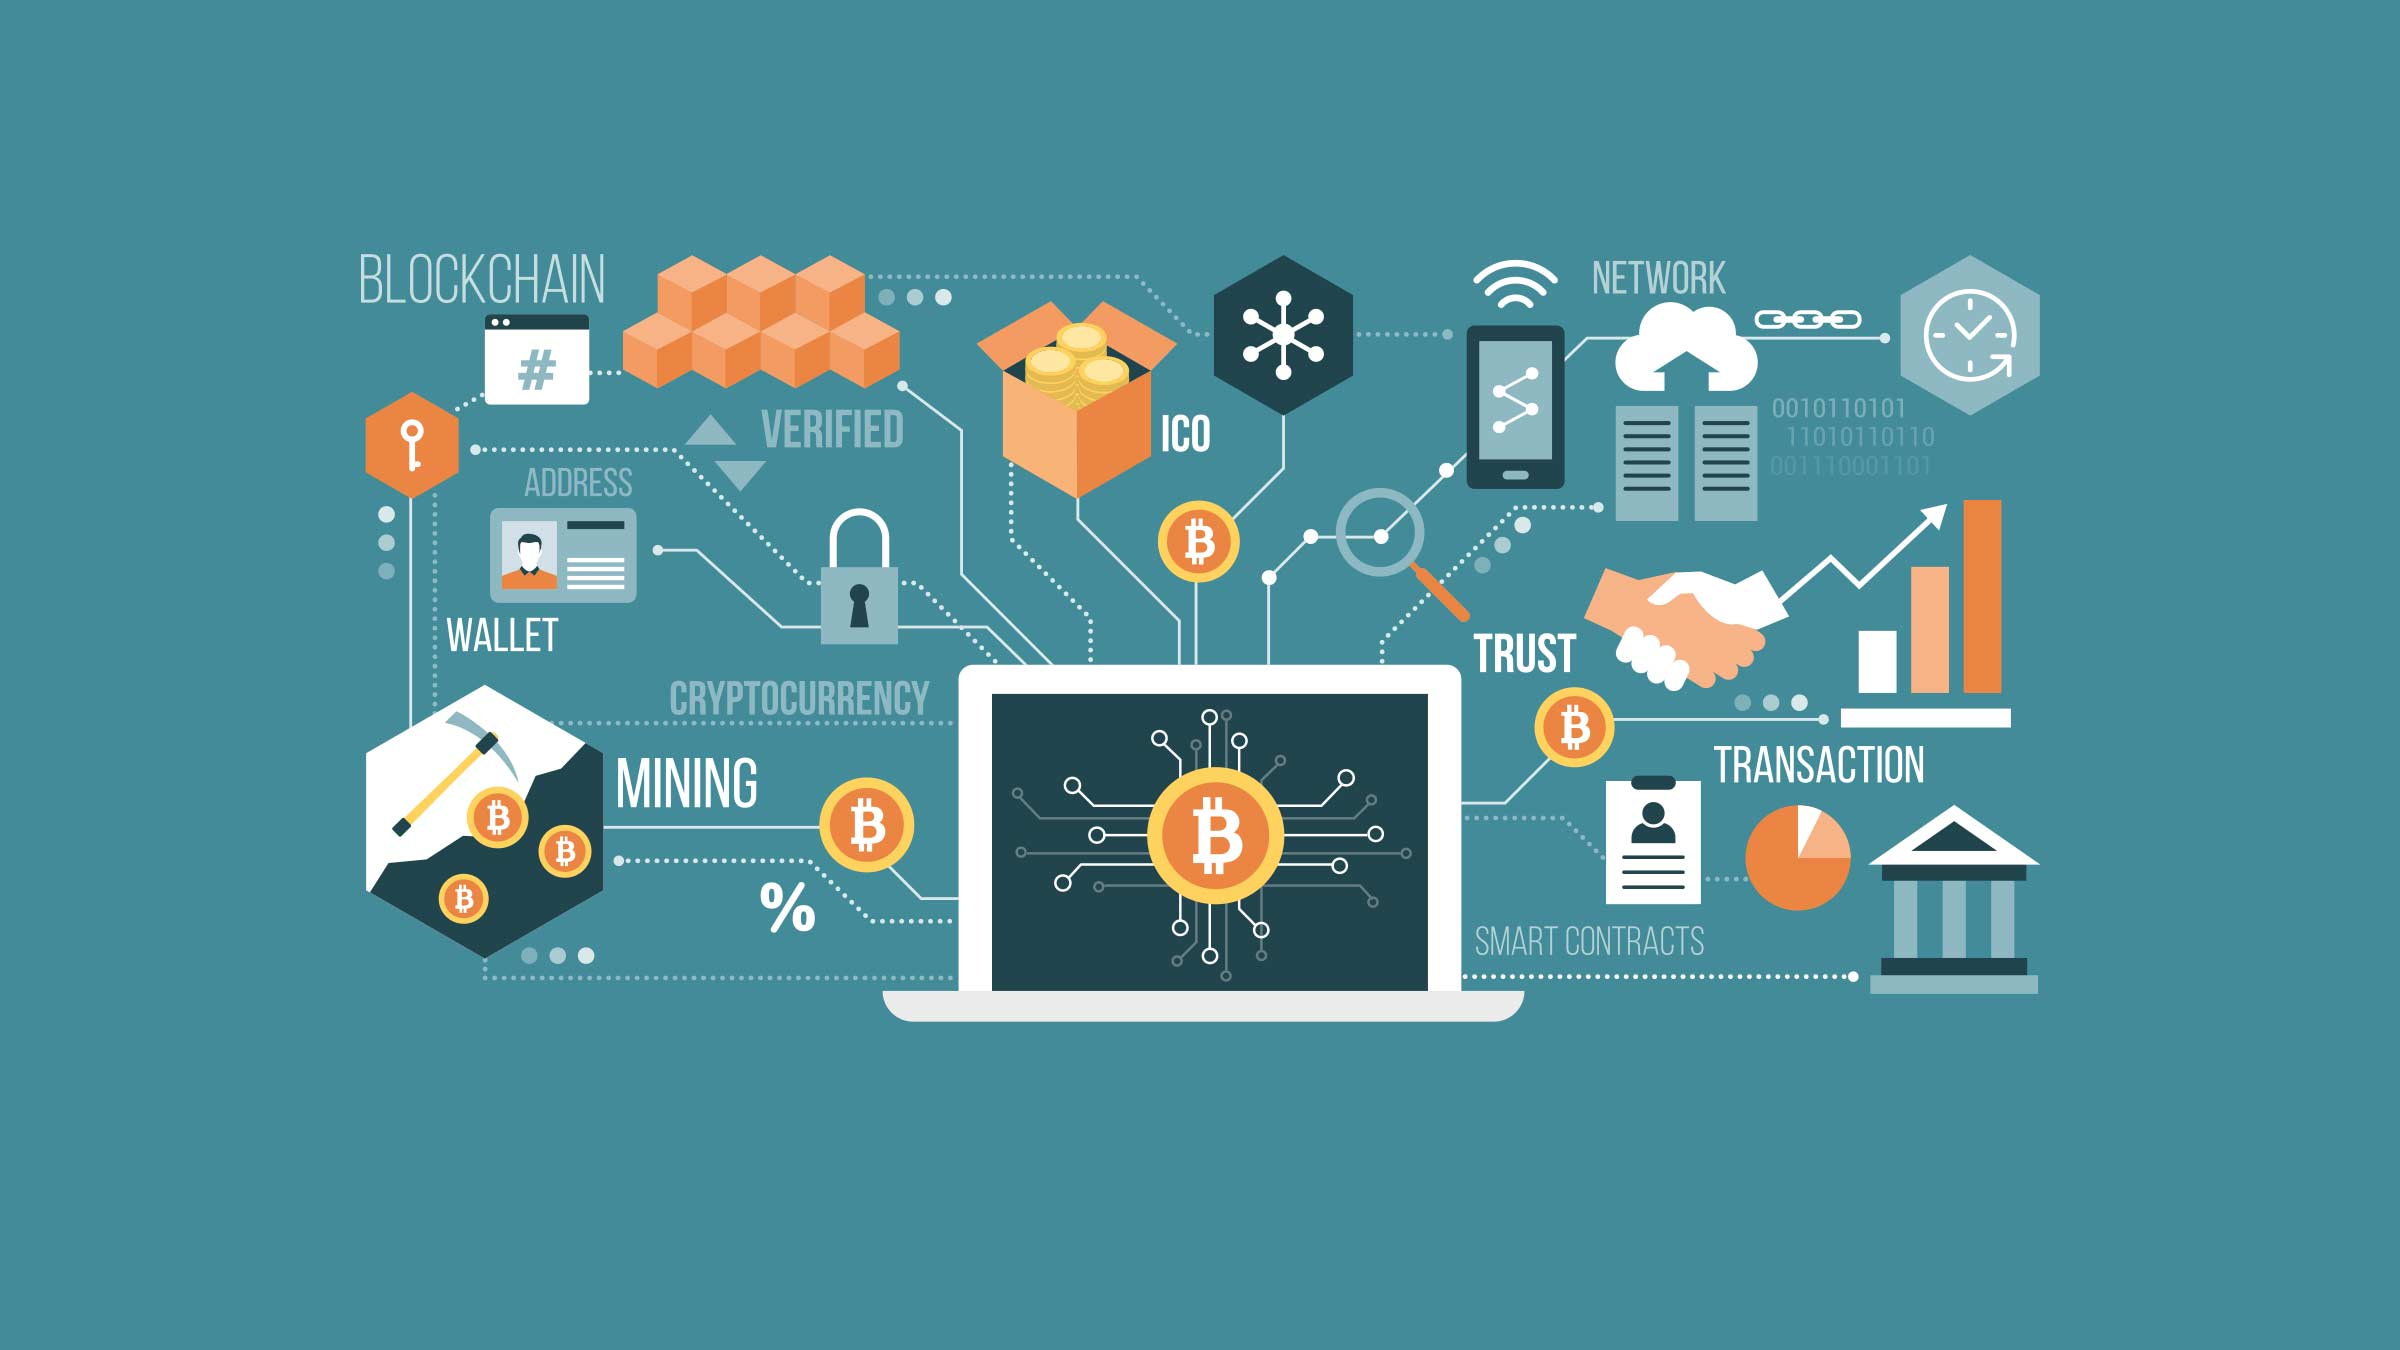
\includegraphics[width=0.75\textwidth]{./img_src/bitcoin.jpg}
\end{center}
\caption{Overview of BitCoin Technology (BCTs).}
\end{figure}

\begin{enumerate}
\item Probable bitcoin consensus mechanism
\item Paxos (Part-Time Parliament) consensus mechanism~\cite{paxos_made_easy, paxos_made_practical}
\item Raft consensus mechanism~\cite{raft_extd}
\end{enumerate}

Bitcoins one is probably the simplest one, but having bugs. The Paxos allows different types of sources and faults to come, it learns and fixes it. Raft does not allow any fault to happen.

The basic overall way in which consensus happen in bitcoin might be the following,

\begin{enumerate}
\item The transaction comes to server from client nodes;
\item Server stores that in file system database as unverified transaction;
\item At the point of interval of 10 minutes server broadcasts it to the miners network i.e. to every miner;
\item Each miner individually verifies and adds correct transaction in a block. Each node holds its block creation and validates the new block as soon as it gets new block from network. Who's block is valid and introduced first to network will be added to everyone's chain and they will start making new block on top of it. Sometimes forks might be created for the networking distance between distant nodes, at that moment conflict will come. If a new introduced block's previous hash does not match with the last block's current hash the node requests to the network to get the missing blocks one by one until the blocks match, it validates it, delete the wrong blocks (make them orphan) and add missing blocks to own chain to resolve fork and maintain longest updated chain. So it is a race between miner nodes.
\item Server gets a copy from miners group and updates own copy and delete the added tansactions from file system.
\end{enumerate}

\subsection{Applications of BCTs}
Block-Chain Technology provides one major advantage over conventional centralized database system: immunity from unexpected data changes or Hacks, which gives rise to numerous applications. Some of them include

\begin{itemize}
\item Crypto-currency: Creating and transferring digital money, Data Mining.
\item Military applications: Secure and verified records of Every Military Events and documents.
\item Structural health Monitoring
\item e-Biding Systems
\item Election System or e-Voting Systems
\item Selling Records and other Commercial Applications
\item Music Copyright Verification System
\item Integrity Analysis of Media Files
\end{itemize}

\subsection{Security and Integrity in BCTs}
As the data is not sitting on a single data server so there is no security issue for Server Hacking. And also the hash-Chain with Cryptography makes it near to impossible to figure out or change previous data block in the blockchain. Before adding any data block with the help of consensus mechanism the blocks are verified with the digital signature of the node and some solution of nonce (the number of times the cllient application required to calculate the mathematical problem) and various other meta data.
As in some interval the system is refreshing itself, if some error seems to be occured, it backs up itself by contacting the miners (the trusted nodes), compare their files and back up with the valid one. So no integrity problem is there, unless and until the internet works fine.
